% Coaxial Autogyro Stack — Technical Schematic
% Compile: pdflatex stacked_autogyro.tex
\documentclass[tikz,border=18pt]{standalone}
\usepackage{amsmath}
\usepackage{amssymb}
\usepackage{tikz}
\usetikzlibrary{angles,quotes,arrows.meta,calc,decorations.pathreplacing,patterns,positioning}

\begin{document}
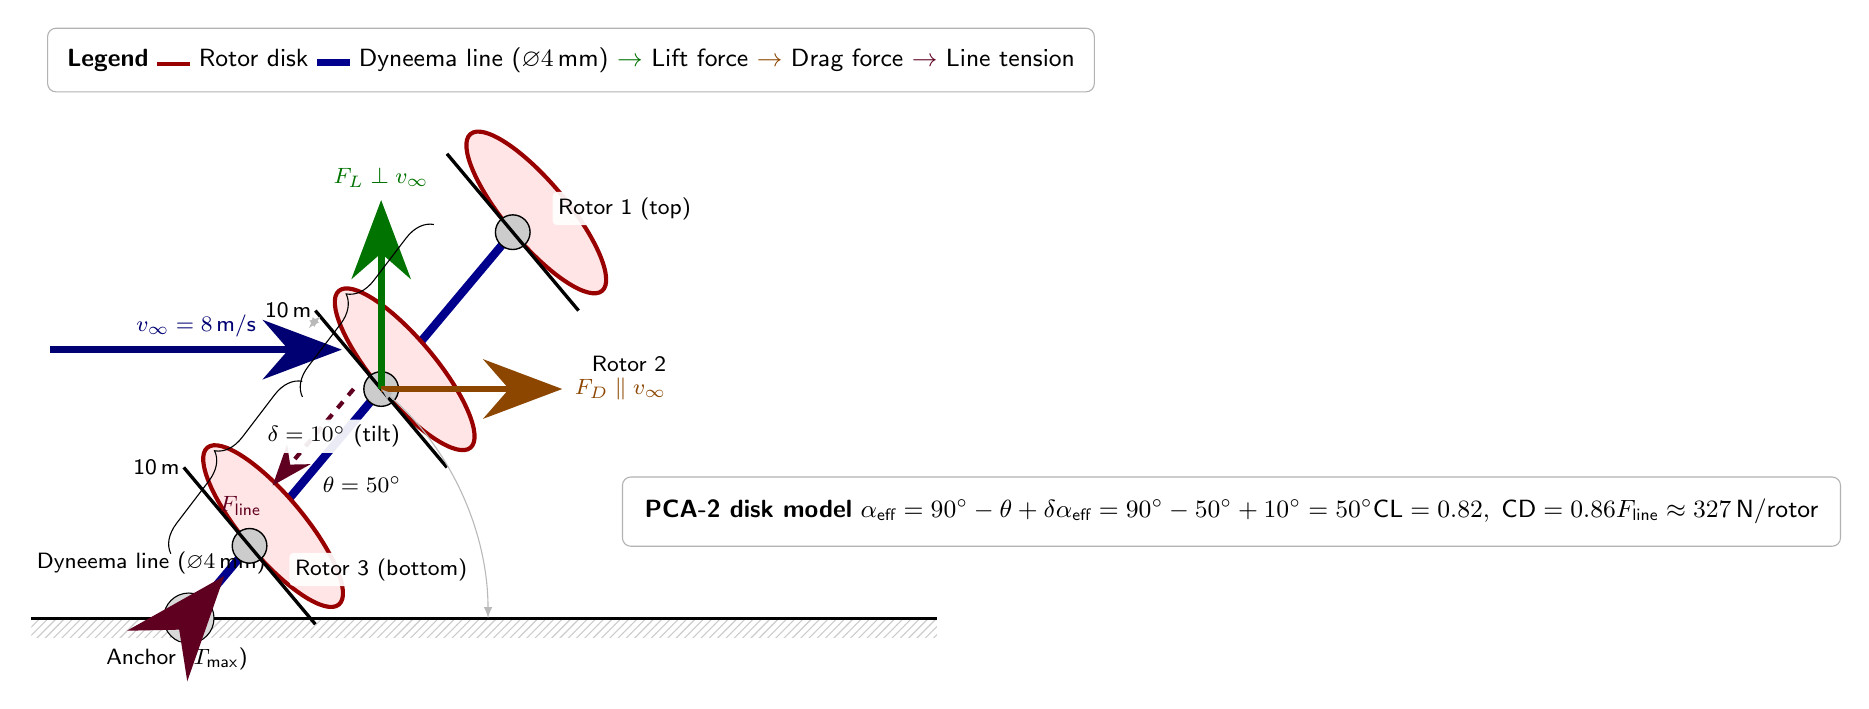
\begin{tikzpicture}[
    scale=1.0,
    tline/.style={draw=blue!55!black, line width=3.0pt},
    force/.style={-{Stealth[scale=2.0]}, line width=2.5pt},
    forcecomp/.style={-{Stealth[scale=1.5]}, line width=1.5pt, dashed},
    annot/.style={font=\footnotesize\sffamily, fill=white, fill opacity=0.92,
                  text opacity=1, inner sep=2pt, rounded corners=1.5pt},
    annotplain/.style={font=\footnotesize\sffamily},
    rotor/.style={draw=red!60!black, fill=red!10, line width=1.5pt},
    dimension/.style={latex-latex, thin, draw=gray!55},
]

\def\lineangle{50}
\def\tiltangle{10}
\def\rotorradius{1.3}
\def\spacing{2.6}

% Anchor point
\coordinate (A) at (1.5, 0);
\coordinate (Ldir) at ({cos(\lineangle)}, {sin(\lineangle)});

% Rotor positions — top rotor terminates the line
\coordinate (R1) at ($(A) + 1.2*(Ldir)$);      % bottom
\coordinate (R2) at ($(R1) + \spacing*(Ldir)$); % middle
\coordinate (R3) at ($(R2) + \spacing*(Ldir)$); % top — line terminates here

% Ground
\fill[pattern=north east lines, pattern color=black!20] (-0.5,-0.25) rectangle (11,0);
\draw[line width=1pt] (-0.5,0) -- (11,0);

% Anchor
\filldraw[fill=gray!30, draw=black] (A) circle (0.32);
\node[annot, below=0.3cm of A, xshift=-0.15cm] {Anchor ($T_{\text{max}}$)};

% Kite line — terminates at top rotor R3 (no free end)
\draw[tline] (A) -- (R3);
\node[annotplain] at ($(A)!0.55!(R1) + (-0.9, 0.2)$)
    {Dyneema line ($\varnothing 4$\,mm)};

% Wind arrow
\draw[force, blue!45!black]
    ($(R2) + (-4.2, 0.5)$) -- ($(R2) + (-0.5, 0.5)$)
    node[midway, above, annotplain] {$v_\infty = 8\,\text{m/s}$};

% Rotor 1 (top — terminates the line)
\begin{scope}[shift={(R3)}]
    \pgfmathsetmacro{\diskangle}{\lineangle + 90 - \tiltangle}
    \fill[rotor, rotate=\diskangle] (0, -\rotorradius*0.3) ellipse ({\rotorradius} and {\rotorradius*0.3});
    \filldraw[fill=gray!40, draw=black, line width=0.5pt] (0,0) circle (0.22);
    \draw[line width=1.2pt, rotate=\diskangle] (-\rotorradius, 0) -- (\rotorradius, 0);
\end{scope}
\node[annot, right=0.5cm of R3, yshift=0.3cm] {Rotor 1 (top)};

% Rotor 2 (middle)
\begin{scope}[shift={(R2)}]
    \pgfmathsetmacro{\diskangle}{\lineangle + 90 - \tiltangle}
    \fill[rotor, rotate=\diskangle] (0, -\rotorradius*0.3) ellipse ({\rotorradius} and {\rotorradius*0.3});
    \filldraw[fill=gray!40, draw=black, line width=0.5pt] (0,0) circle (0.22);
    \draw[line width=1.2pt, rotate=\diskangle] (-\rotorradius, 0) -- (\rotorradius, 0);
\end{scope}
\node[annot, above right=0.15cm and 2.6cm of R2] {Rotor 2};

% Rotor 3 (bottom)
\begin{scope}[shift={(R1)}]
    \pgfmathsetmacro{\diskangle}{\lineangle + 90 - \tiltangle}
    \fill[rotor, rotate=\diskangle] (0, -\rotorradius*0.3) ellipse ({\rotorradius} and {\rotorradius*0.3});
    \filldraw[fill=gray!40, draw=black, line width=0.5pt] (0,0) circle (0.22);
    \draw[line width=1.2pt, rotate=\diskangle] (-\rotorradius, 0) -- (\rotorradius, 0);
\end{scope}
\node[annot, right=0.5cm of R1, yshift=-0.3cm] {Rotor 3 (bottom)};

% Force vectors on middle rotor
\draw[force, green!45!black] (R2) -- ++(0, 2.4)
    node[above, annotplain, green!45!black] {$F_L \perp v_\infty$};
\draw[force, orange!55!black] (R2) -- ++(2.3, 0)
    node[right, annotplain, orange!55!black] {$F_D \parallel v_\infty$};
\draw[forcecomp, purple!50!black] ($(R2) + (-0.35, 0)$) -- ++($-1.6*(Ldir)$)
    node[below left, annotplain, purple!50!black] {$F_{\text{line}}$};

% Line angle arc
\coordinate (HorizArc) at ($(A) + (3.8, 0)$);
\draw[dimension] (HorizArc) arc[start angle=0, end angle=\lineangle, radius=3.8cm];
\node[annot] at ($(A) + (2.2, 1.7)$) {$\theta = 50^\circ$};

% Disk tilt arc
\begin{scope}[shift={(R2)}]
    \pgfmathsetmacro{\diskangle}{\lineangle + 90 - \tiltangle}
    \coordinate (PerpLine) at ({-sin(\lineangle)*1.2}, {cos(\lineangle)*1.2});
    \draw[dimension] (PerpLine) arc[start angle={\lineangle+90}, end angle={\diskangle}, radius=1.2cm];
    \node[annot] at ({-sin(\lineangle+90-\tiltangle/2)*0.85}, {cos(\lineangle+90-\tiltangle/2)*0.85})
        {$\delta = 10^\circ$ (tilt)};
\end{scope}

% Tension indicator near anchor
\draw[force, purple!50!black, line width=3.5pt] ($(A) + 0.2*(Ldir)$) -- ++($0.5*(Ldir)$);

% Section lengths
\draw[decorate, decoration={brace, amplitude=10pt}]
    ($(R1) + (-1.0, -0.1)$) -- ($(R2) + (-1.0, 0.1)$)
    node[midway, left=0.6cm, annotplain] {10\,m};
\draw[decorate, decoration={brace, amplitude=10pt}]
    ($(R2) + (-1.0, -0.1)$) -- ($(R3) + (-1.0, 0.1)$)
    node[midway, left=0.6cm, annotplain] {10\,m};

% PCA-2 reference box
\node[draw=black!30, fill=white, rounded corners=3pt, inner sep=8pt,
      anchor=north west, font=\small\sffamily]
    at (7.0, 1.8) {
    \textbf{PCA-2 disk model} \\[3pt]
    $\alpha_{\text{eff}} = 90^\circ - \theta + \delta$ \\
    $\alpha_{\text{eff}} = 90^\circ - 50^\circ + 10^\circ = 50^\circ$ \\
    $\text{CL}=0.82,\; \text{CD}=0.86$ \\
    $F_{\text{line}} \approx 327\,\text{N/rotor}$
};

% Legend
\node[draw=black!30, fill=white, rounded corners=3pt, inner sep=7pt,
      anchor=north west, font=\small\sffamily]
    at (-0.3, 7.5) {
    \textbf{Legend} \\[2pt]
    \textcolor{red!60!black}{\rule{12pt}{1.5pt}} Rotor disk \\[1pt]
    \textcolor{blue!55!black}{\rule{12pt}{2.5pt}} Dyneema line ($\varnothing 4$\,mm) \\[1pt]
    \textcolor{green!45!black}{$\rightarrow$} Lift force \\[1pt]
    \textcolor{orange!55!black}{$\rightarrow$} Drag force \\[1pt]
    \textcolor{purple!50!black}{$\rightarrow$} Line tension
};

\end{tikzpicture}
\end{document}
